
\chapter{Introduction}

In 2008, Satoshi Nakamoto invented \bitcoin and the concept of {\em blockchains}~\cite{bitcoin}. Since then, blockchains have attracted considerable interest for their applications in cross-border payments~\cite{hileman2017global,kazan2015value}, digital contracts~\cite{cong2019blockchain,wust2018you,pilkington201611} and more. At the heart of \bitcoin and many other blockchain projects is the {\em Nakamoto longest chain protocol}. It enables an open (permissionless) network of nodes to reach consensus on an ordered log of transactions and is tolerant to Byzantine adversarial attacks with no more than 50\% of the compute power in the network. To achieve this high level of security, however, the longest chain protocol severely limits transaction throughput and latency  (\S\ref{sec:background}). \bitcoin, for example, supports 3--7 transactions per second and can take hours to confirm a transaction with a high level of reliability~\cite{bitcoin}.  

%Today's cryptocurrencies have poor transaction throughput and slow confirmation times. Bitcoin supports 3--7 transactions per second and can take hours to confirm a transaction with a high level of reliability~\cite{bitcoin}.  The root cause for this poor performance is the {\em Nakamoto longest chain protocol} (\S\ref{sec:background}), a Byzantine fault-tolerant consensus protocol that lies at the heart of Bitcoin and many other cryptocurrencies~\cite{buterin2016ethereum, citeothers}. Roughly speaking, the longest chain protocol enables an open (permissionless) network of nodes to reach consensus on an ordered log of transactions, provided that at least 50\% of the compute power in the network belongs to honest nodes that follow protocol. 

The limitations of the longest chain protocol have led to a flurry of work in recent years on more scalable blockchain consensus protocols (\S\ref{sec:related} discusses related work). However, until recently, no protocol has been shown to guarantee Bitcoin-level security (up to 50\% adversarial power) as well as high throughput and low latency. Prism~\cite{prism-theory} is the first such protocol. Prism is a Proof-of-Work (PoW) blockchain consensus protocol that is  (1) secure against 50\% adversarial compute power, (2) can achieve optimal throughput (up to the network communication bandwidth), and (3) can achieve near-optimal confirmation latency (on the order of the network's propagation delay). Prism removes the throughput and latency limitations of the longest chain protocol by systematically decoupling security and throughput in the blockchain  (\S\ref{sec:overview}).  
%transaction proposal, validation, and confirmation in the blockchain (\S\ref{sec:overview}). 
A recent theoretical paper described the core protocol and analyzed its security properties~\cite{prism-theory}.

While these theoretical results are promising, it is not clear how well they can translate into real-world performance. First, the \prism consensus protocol is much more complex than the longest chain protocol: clients must maintain over 1000 distinct blockchains, which refer to each other to create an intricate directed acyclic graph (DAG) structure, and they must process blocks at very high rates (e.g., 100-1000s of blocks per second at 100s of Mbps) to update these blockchains and confirm transactions. Second, Prism's theoretical analysis relies on several simplifying assumptions (e.g., round-based synchronous communication and a simple network model that ignores queuing delay), and to make the analysis tractable, the performance bounds are specified up to large constants that may not be indicative of real-world performance. Third, Prism's theory focuses on the network as the primary performance bottleneck, but a real high-throughput blockchain system must overcome other potential performance bottlenecks. For example, in addition to achieving consensus on a transaction order, clients must also {\em execute} transactions and maintain the {\em state} of the ledger to confirm transaction. Though some academic prototypes ignore transaction execution (e.g., \cite{ohiecode, conflux}),
%\cite{cite-codebases-better-than-papers},
in practice, it often turns out to be the bottleneck due to its high I/O overhead, c.f.,~\cite{raju2018mlsm},  \S\ref{sec:eval-resource}.
Finally, Prism could be vulnerable to spamming, a practical security concern that has not been fully analyzed. 


% the performance of a blockchain system depends on more than the consensus protocol. The consensus protocol orders transactions, but to confirm them, the client must {\em execute} the transactions in order and keep track of the {\em state} of the ledger. 




In this thesis, we present the design (\S\ref{sec:design}) and  implementation (\S\ref{sec:implementation}) of a Bitcoin-like system based on the \prism consensus protocol. Our implementation features payments as multi-input-multi-output transactions (payments) similar to pay-to-public-key (P2PK) in Bitcoin and Algorand~\cite{algorand, algorandcode}. We evaluate our system on a testbed of up to 1000 EC2 Virtual Machines connected via an emulated wide area network. Figure \ref{fig:compare} summarizes the results. \prism consistently achieves a throughput of over 70,000 tps for a range of security levels $\beta$ denoting the fraction of adversarial compute power.  To guarantee a reversal probability of less than $10^{-9}$, \prism's latency ranges from 13 seconds against an adversary of power $\beta = 20\%$, to $296$ seconds for $\beta = 44\%$. To our knowledge, this makes our system the fastest  implementation of a blockchain system with Bitcoin-level security guarantees. Compared to the longest chain protocol, \prism provides about 10,000$\times$ higher throughput and 1,000$\times$ lower latency. Compared to Algorand~\cite{algorand}, the state-of-the-art proof-of-stake system, \prism achieves 70$\times$ the throughput with about 10 seconds higher latency, and can provide a higher level of security  (up to $\beta = 50\%$ vs. $\beta=33\%$ for Algorand).

\begin{figure} 
    \centering
    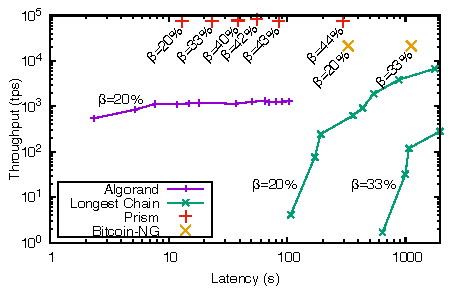
\includegraphics[width=0.75\textwidth]{figures/compare-fig.pdf}
    \caption[Throughput and confirmation latency of Prism, Algorand, Bitcoin-NG, and the longest chain protocol on the same testbed.]{Throughput and confirmation latency of \prism, \algorand, \bng, and the longest chain protocol on the same testbed. Note that the axes are on log scales. For \algorand and the longest chain protocol, parameters are tuned to span an optimized tradeoff between throughput and latency at a given security level. For \bng and \prism, throughput and latency are decoupled so one can simultaneously optimize both at one operating point for a given security level. However, the throughput of Bitcoin-NG drops to that of the longest chain protocol under attack, while that of \prism remains high. More details in \S\ref{sec:related} and \S\ref{sec:eval-performance}. }
    \label{fig:compare}
\end{figure}

We make the following contributions:
\begin{itemize}
    \item We implement a Prism client in roughly 10,000 lines of {\tt Rust} code, and quantify its performance in extensive experiments on EC2. Our result validate Prism's core modeling decisions and theory by showing that it can scale both throughput and latency of the longest chain protocol (without compromising security) in a practical setting. Our code is available here~\cite{prismcode}.
    
    \item Our implementation highlights several performance optimizations, e.g., asynchronous ledger updates, and a scoreboarding technique that enables parallel transaction execution without race conditions (see ~\S\ref{sec:implementation-highlights}). We show that with these careful optimizations, it is possible to alleviate CPU performance bottlenecks and provide linear CPU scaling up to at least 8 cores. At this point, the primary bottleneck for our implementation is the underlying database (RocksDB~\cite{rocksdb} and I/O to the SSD persistent storage). This suggests that future research on databases optimized for blockchain-specific access patterns could further improve performance. 
    
    \item We evaluate practical security concerns like censorship attack, balancing attack, and spamming (see ~\S\ref{sec:eval-attack}). Additionally, we propose a simple solution to the spamming problem that reduces spam traffic by 80\% while only adding 5 seconds to the confirmation delay. Our implementation illustrates that \prism performs well even under these attacks, and makes a stronger case for the practical viability of the system.
    
\end{itemize}

%Our implementation and evaluation provide several key takeaways. First, our results validate Prism's core modeling and design decisions in a practical setting by demonstrating that it can scale both throughput and latency of the longest chain protocol independently of one another without compromising the security guarantee. Second, our implementation shows that with careful performance optimization (see ~\S\ref{sec:implementation-highlights}), it is possible to alleviate CPU performance bottlenecks and provide linear CPU scaling up to \ma{XXX cores}. At this point, the primary bottleneck for our implementation is the underlying database (RocksDB~\cite{rocksdb} and I/O to persistent storage (SSDs)). Therefore future research on databases optimized for blockchain-specific access patterns could provide further performance improvements. 


% e.g., asychoronous ledger updates, and a scoreboarding technique that enables parallel transaction execution without race conditions. We show that these optimizations alleviate CPU performance bottlenecks and provide linear CPU scaling, such that the primary bottleneck is the underlying database (RocksDB~\cite{rocksdb} and I/O to persistent storage (SSDs)). Further performance improvements may therefore be possible by optimizing the database.

The rest of the thesis is organized as follows. In \S\ref{sec:related} we discuss different scaling approaches taken in blockchains. In \S\ref{sec:background} we discuss the longest chain protocol and its limitations to motivate the design of the \prism protocol in \S\ref{sec:overview} and \S\ref{sec:design}. We discuss the details of the client implementation with an interface enabling pay-to-public-key transactions in \S\ref{sec:implementation}. Evaluations are presented in \S\ref{sec:eval} to assess the impact of network resources (bandwidth, topology, propagation delay) and computation resources (memory, CPU) on the overall performance. \S\ref{sec:conclusion} concludes the thesis.


%%a host of related topics of core interest to the blockchain ecosystem; this includes interfacing Prism to a smart contract programming layer, introduction of light clients (which are simply interested in making and validating specific transactions) and bootstrapping new Prism clients into a running system - each of these is a future direction of research of great interest.


\if 0

% TODO: do we include performance here? Tell the performance first or explain the protocol first?

% TODO: if to compare the performance, what are the baselines? How to compare (cite numbers, run experiments, if so, do we need to optimize their code?) For some of them, modify Prism client into our impelmentation. For algorand, run their code. But what if their implementation is flawed? Explain the results we got (cause of the bottleneck), understand their bottleneck.

% comparisons: Algorand (fame, it could be that their paper is not doing real transactions. use their real code and try to reproduce the number in the paper), Bitcoin (longest chain), OHIE (parallel chain). Remember to point out the security level. This is FINAL.
% mentions: HotStuff
% Point that Conflux is copy cat
% Use Prism 1.0 to help rationale the protocol in Design section.
% Make other system actually do transactions

% Scale of the evaluation
% Hope that the scalability curves are flat, so that reader can assume the scalability (we could provide a breakdown of the CPU/IO resource spent)

% Mention that we have included all possible functions of the client so it is real.

% TODO: make full use of the code. Change parameters to show the idea of other systems.

Text...

Takeaways from experiments. Maybe insert a figure here. % TODO: possibilities: throughput - latency, different protocols take different positions (curve for parameterized ones)

% other potential comparisons: Conflux, Prism 1.0, Bitcoin-NG



Figure 1: comparison of throughput and latency with other blockchain protocols: 

Algorand - best permissionless PoS BFT protocol

longest chain - the original blockchain protocol (frontier as we vary mining rate and block size)

Ohie - parallel chain protocol (give state execution for free)

Prism - our protocol

Network setting (first draft)

100 nodes

artificial delay 300 ms per hop (exponential)

network bandwidth: whatever is sufficient for Prism to achieve 100K Tps. (around 200 to 300Mbps)


\fi
